

\documentclass[journal]{IEEEtran}
%
% If IEEEtran.cls has not been installed into the LaTeX system files,
% manually specify the path to it like:
% \documentclass[journal]{../sty/IEEEtran}


\usepackage{amsthm, array}
\usepackage{amssymb}
\usepackage{amsfonts}
\usepackage{epsfig}
\usepackage{url}
\usepackage{multirow}
\usepackage{subfigure}
\usepackage{listings}
\usepackage{verbatim}
\usepackage{color}
\usepackage[normalem]{ulem}
\usepackage{booktabs}
\usepackage{pgfplots}
\usepackage{hhline}
\usepackage{tabu}
\usepackage{tcolorbox}
\usepackage{tikz}
\usepackage[cmex10]{amsmath} % Use the [cmex10] option to ensure complicance
% with IEEE Xplore (see bare_conf.tex)

\newcommand{\bbe}{\mathbb{E}}
\newcommand{\pa}{\mathcal{P}_{\rm A}}
\newcommand{\beq}{\begin{equation}}
\newcommand{\eeq}{\end{equation}}
\newcommand{\bi}{\begin{enumerate}}
	\newcommand{\ei}{\end{enumerate}}
\newcommand{\bea}{\begin{eqnarray}}
\newcommand{\eea}{\end{eqnarray}}
\newcommand{\bc}{\begin{center}}
	\newcommand{\ec}{\end{center}}
\newcommand{\denotes}{\stackrel{\triangle}{=}}
\newcommand{\la}{\langle}
\newcommand{\ra}{\rangle}
\newcommand{\nn}{\nonumber}
\newcommand{\bPsi}{{\mbox {\boldmath $\Psi$}}}
\newcommand{\her}{{\scriptscriptstyle H}}
\newcommand{\thetemp}{\fnsymbol{temp}}
\newcommand{\cI}{\mathcal{I}}
\newcommand{\cT}{\mathcal{T}}
\newcommand{\cS}{\mathcal{S}}
\newcommand{\at}{{\mathcal{A}_1}}
\newtheorem*{theorem}{\bf Theorem}
\newtheorem*{corollary}{\bf Corollary}
\newtheorem*{definition}{Definition}

\newcommand{\microns}{$\mu$m}
\newcommand{\degrees}{$^{\circ}$}
\newcommand{\Ohms}{\Omega}
\newcommand{\cb}{\color{blue}}
\renewcommand{\qedsymbol}{$\blacksquare$}
\newcommand*{\vertbar}{\rule[-1ex]{0.5pt}{2.5ex}}
\newcommand*{\horzbar}{\rule[.5ex]{2.5ex}{0.5pt}}

\newlength\figureheight
\newlength\figurewidth

\IEEEoverridecommandlockouts

\newcommand{\revision}[1]{\textcolor{black}{#1}}
\newcommand{\myrevision}[1]{\textcolor{red}{#1}}

\hyphenation{op-tical net-works semi-conduc-tor}


\begin{document}
\title{A Novel Clustering Technique Using Backscattering Side Channel for Hardware Trojan Detection}
\author{Luong N. Nguyen,~\IEEEmembership{Student Member,~IEEE}, Baki Berkay Yilmaz~\IEEEmembership{Student Member,~IEEE},  Milos Prvulovic,~\IEEEmembership{Senior Member,~IEEE}, and Alenka Zaji\'{c},~\IEEEmembership{Senior Member,~IEEE}
	%This work has been supported, in part, by NSF grants 1651273 and 1740962 and ONR grant N00014-17-1-2540. The views and findings in this paper are those of the authors and do not necessarily reflect the views of NSF and ONR.}
	%\thanks{Luong N. Nguyen, Chia-Lin Cheng, and Alenka Zaji\'{c} are with the School of Electrical and Computer Engineering, Georgia Institute of Technology, Atlanta, GA 30332, USA, and Milos Prvulovic is with the School of Computer Science, Georgia Institute of Technology, Atlanta, GA 30332, USA.}
}
\maketitle

\begin{abstract}
Due to various factors including time-to-market and cost reduction demands, and the increased complexity of integrated circuit (IC), IC companies tend to get their chip fabricated in offshore foundries. As a results, malicious hardware modifications, a.k.a. hardware Trojans, inserted at untrusted foundries have emerged as a major security concern. Among proposed hardware Trojan detection techniques, reverse engineering based ones appear to be the most accurate and reliable ones that work for all circuits and Trojan types. However, reverse engineering is an extremely expensive, time consuming, and destructive process that prevents these technique to be applied for a large population of ICs in real test environments. This paper proposes a novel clustering method using backscattering side-channel without having a golden chip or any priori knowledge of the chip circuitry to make the deployment of reverse engineering detection possible in large testing scenarios. We create real a testing environment by implementing multiple Trojan benchmarks on a set of 100 boards. The results show that our technique can tolerate manufacturing variations among hardware instances to cluster all boards correctly for not only 9 different dormant Trojan designs on 3 different benchmark circuits from Trusthub \cite{shakya2017benchmarking}, but also dormant Trojan designs whose size is sunken to as small as 0.33 \% of the original circuit.

\end{abstract}

% Note that keywords are not normally used for peerreview papers.
\begin{IEEEkeywords}
Hardware Trojan, Hardware security, hardware trust,                                                                                                                                                        Backscattering side channel, Trojan detection.
\end{IEEEkeywords}

\section{Introduction}
Over the past few years, we saw a shift in the manufacturing model and design flow of integrated circuit (IC) companies due to various factors including time-to-market and cost reduction demands, and the increased complexity of ICs. Today, IC companies have fully adopted the ”horizontal model” in which they use IPs from third-party companies and outsource all hardware fabrication to offshore foundries. While the new design flow model allows them to tremendously reduce the
cost, time-to-market and fabrication errors, it significantly reduces the level of trust of the hardware. As a result, malicious hardware changes, a.k.a. hardware Trojans (HT), have emerged as a major security concern because the hardware provides the base layer of security and trust that all software layers depend and build on. A typical HT consists of two parts: the trigger and payload. The trigger is a circuit that constantly checks for the right conditions to activate the Trojan and the payload is the entire malicious function that the Trojan executes when it is triggered. Typically, HTs get triggered by very rare conditions, making them extremely challenging to detect by traditional function verification and testing.

HTs could be injected into an IC by adversaries at any stage of its design and fabrication flow. Fig \ref{fig:adversaries} shows the IC life cycle and a subset of opportunities for inserting HTs into the IC, in which inserting HTs at the foundry is the most common scenario because IC companies tend to get their chip fabricated in offshore foundries, which are harder to ensure  the level of trust, for the sake of cost reduction. As a result,  numerous HT detection techniques focusing on detecting HT inserted at the foundry have been proposed and they can be classified into two groups: reverse engineering and side-channel approaches. 

Reverse-engineering techniques rely on devastatingly scanning the actual layout of the IC to re-build the GDSII and netlist level of the chip \cite{torrance2009state}-\nocite{nasr2017efficient,fyrbiak2018hal,7293657,8031551,6783305}\cite{7428081}. The destructive scanning process consists of decapsulation to remove the die from the package, delayering to strip each layer off the die, and imaging to reconstruct images for every layer. After getting the GDSII and netlist level of the chip, these techniques are capable of detect any malicious post-RTL-design insertion with perfect accuracy by comparing them to the GDSII and netlist of a trusted design. However, reverse-engineering is extremely expensive and time-consuming. In addition, all the chips after reverse engineering are destroyed. This is the reason why in spite of being exceedingly accurate and reliable, it is not practical to apply reverse engineering based HT detection techniques for testing a large population of ICs.

Side-channel analysis based approaches rely on measuring some non-functional properties from outside the IC as it operates, and
comparing the measurements to reference signals produced by either simulation \cite{he2017hardware}-\nocite{8064895}\cite{8809738} or a verified genuine device \cite{8701559}. Potential side-channels include backscattering \cite{8701559}, power consumption \cite{agrawal2007trojan}, \cite{banga2008region}, leakage current \cite{7107361}, temperature \cite{bao2015temperature}, electromagnetic emanations (EM) \cite{he2017hardware}, \cite{ngo2016method}, or a combination of multiple side-channels \cite{hu2013high}, \cite{nowroz2014novel}. In some techniques, additional measurement circuitry is added to the design \cite{cha2013trojan}, \cite{lecomte2017chip}, which allows the specific
chosen signals to be measured close to the signal’s source. However, additional circuitry results in circuit size, manufacturing cost, performance, and power overhead. Therefore, the majority of side-channel based detection techniques require no modifications to the chip itself and rely on measuring some side-channel signals from the outside of the chip. In contrast to reverse engineering technques, the side-channel based techniques can be applied to a large population of ICs because side-channel measurements are cheap and fast, and the ICs are not defective after getting tested. However, the problem with side-channel techniques is the dependence on having a golden HT-free chip, which is not a practical assumption if HTs were inserted at foundries, or simulation, which only works for the specific circuits modeled. 

Motivated by the these shortcomings of the both approaches, we propose novel a clustering algorithm using side-channel, as a bridging solution, to categorize a large population of ICs into clusters
based on how HTs (if existed) affect their side-channel signals. With our clustering algorithms, the deployment of reverse engineering techniques to a large population of ICs will be practical because they will only need to reverse-engineer one IC for each cluster to decide if the whole cluster is HT-free or HT-infected. We chose to use the backscattering side-channel, a new physical side-channel that is proved to be a perfect fit and outperforms other side-channels for HT detections \cite{8701559}.

We prototype a real testing enviroment by evaluating our clustering algorithm for multiple HT and circuit benchmark designs over a set of 100 boards, in which each board will be randomly loaded either HT-free or HT infected design. The results show that our technique is capable of clustering all boards correctly for not only 9 different dormant Trojan designs on 3 different benchmark circuits from Trusthub \cite{shakya2017benchmarking}, but also dormant Trojan designs whose size is sunken to as small as 0.31 \% of the original circuit. The following summarized the contribution of our work:
\begin{itemize}
	\item Propose a novel clustering algorithm that is capable of classifying a large population of ICs into clusters based on how HT affects their backscattering side-channel signal without having a verified HT-free (golden) chip or any priori knowledge about circuitry of the chip.
	\item Create a real testing environment including a set of 100 boards implemented multiple HT benchmarks. This huge set of boards allow a thourough evaluation of the manufacturing variation among different hardware instances with enough statistics, which have never been done before.  
\end{itemize}

The rest of the paper is organized as follows. In Section \ref{background}, we give some background for this work. Section \ref{problem} defines the problem and our thread model. Section \ref{agorithm} defines our clustering technique and algorithm, while Section \ref{evaluation} we evaluate the robustness of our algorithm. Finally, Section \ref{conclusion} concludes the paper.

\begin{figure}[tb]	
	\centering
	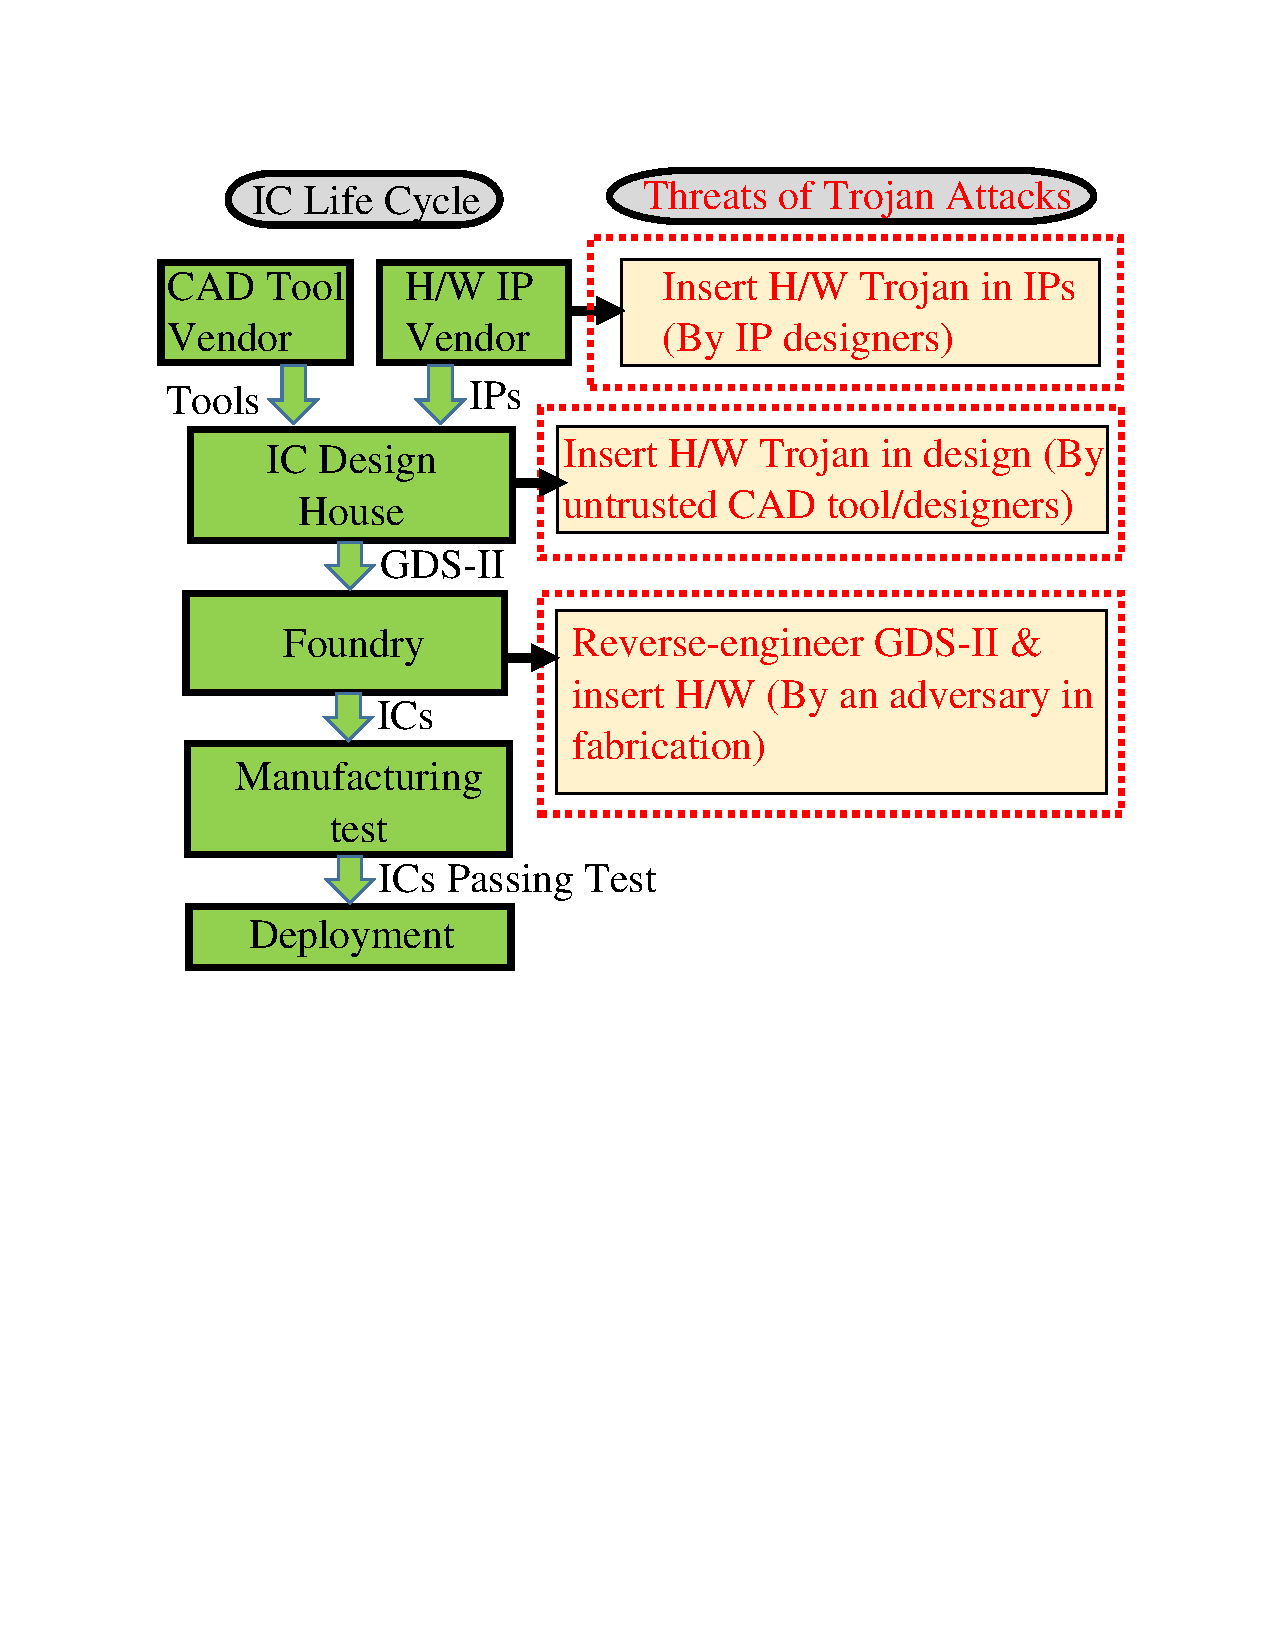
\includegraphics[viewport=0.75in 4.4in 18in 10in, clip,height=2.5in,width=9in,scale=0.5]{figure/HT_attack_model.pdf}
	\caption{IC life cycle with examples of HT insertion activity \cite{bhunia2014hardware}.}%\vspace{-0.2in}
	\label{fig:adversaries}	
\end{figure}
\section{Background}\label{background}
\subsection{Hardware Trojans: Characteristics and Taxonomy}
 Conventionally, hardware had been seen as the root of trust and the only untrusted parts were the software or firmware running on top of the hardware. However, several studies on HTs has proved that even the hardware platform cannot be trusted anymore.  Over the past several years, numerous papers have been published on the topic of understanding the intent and behavior \cite{chakraborty2009hardware,bhunia2014hardware}, implementation \cite{zhang2014detrust}\nocite{chen2008hardware,chakraborty2013hardware}-\cite{shakya2017benchmarking}, and taxonomy of hardware Trojans \cite{shakya2017benchmarking}\nocite{tehranipoor2010survey}-\cite{karri2010trustworthy}. HTs are undesired and unknown malicious modifications to a hardware circuit that have three common characteristics: rarity of activation, malicious purpose, and invasion of detection \cite{bhunia2014hardware}. 
 
 Typically, a HT consists of two components: trigger and payload. The trigger circuit gets input from the host circuit to constantly check for the right conditions to activate the payload. In those very rare conditions, the payload is activated by the triggering signal from the trigger circuit to perform malicious activities. They could be leaking sensitive information, allowing the attackers to gain access to the hardware, or shortening the operational lifetime of the hardware.

As the number and complexity of HTs as increased dramatically, several studies on the topic of characterizing and classifying HTs have been published over the last few years \cite{shakya2017benchmarking}\nocite{tehranipoor2010survey,karri2010trustworthy}-\cite{wang2008detecting}. The most comprehensive work to date is proposed by \cite{shakya2017benchmarking}. Fig. \ref{fig:taxonomy} illustrates different ways of classifying HTs. As shown in the figure, HTs can be classified by their activation mechanism, functionality, inserted location, abstraction level, or the phase in the IC design flow they are inserted.
\begin{figure}[tb]	
	\centering
	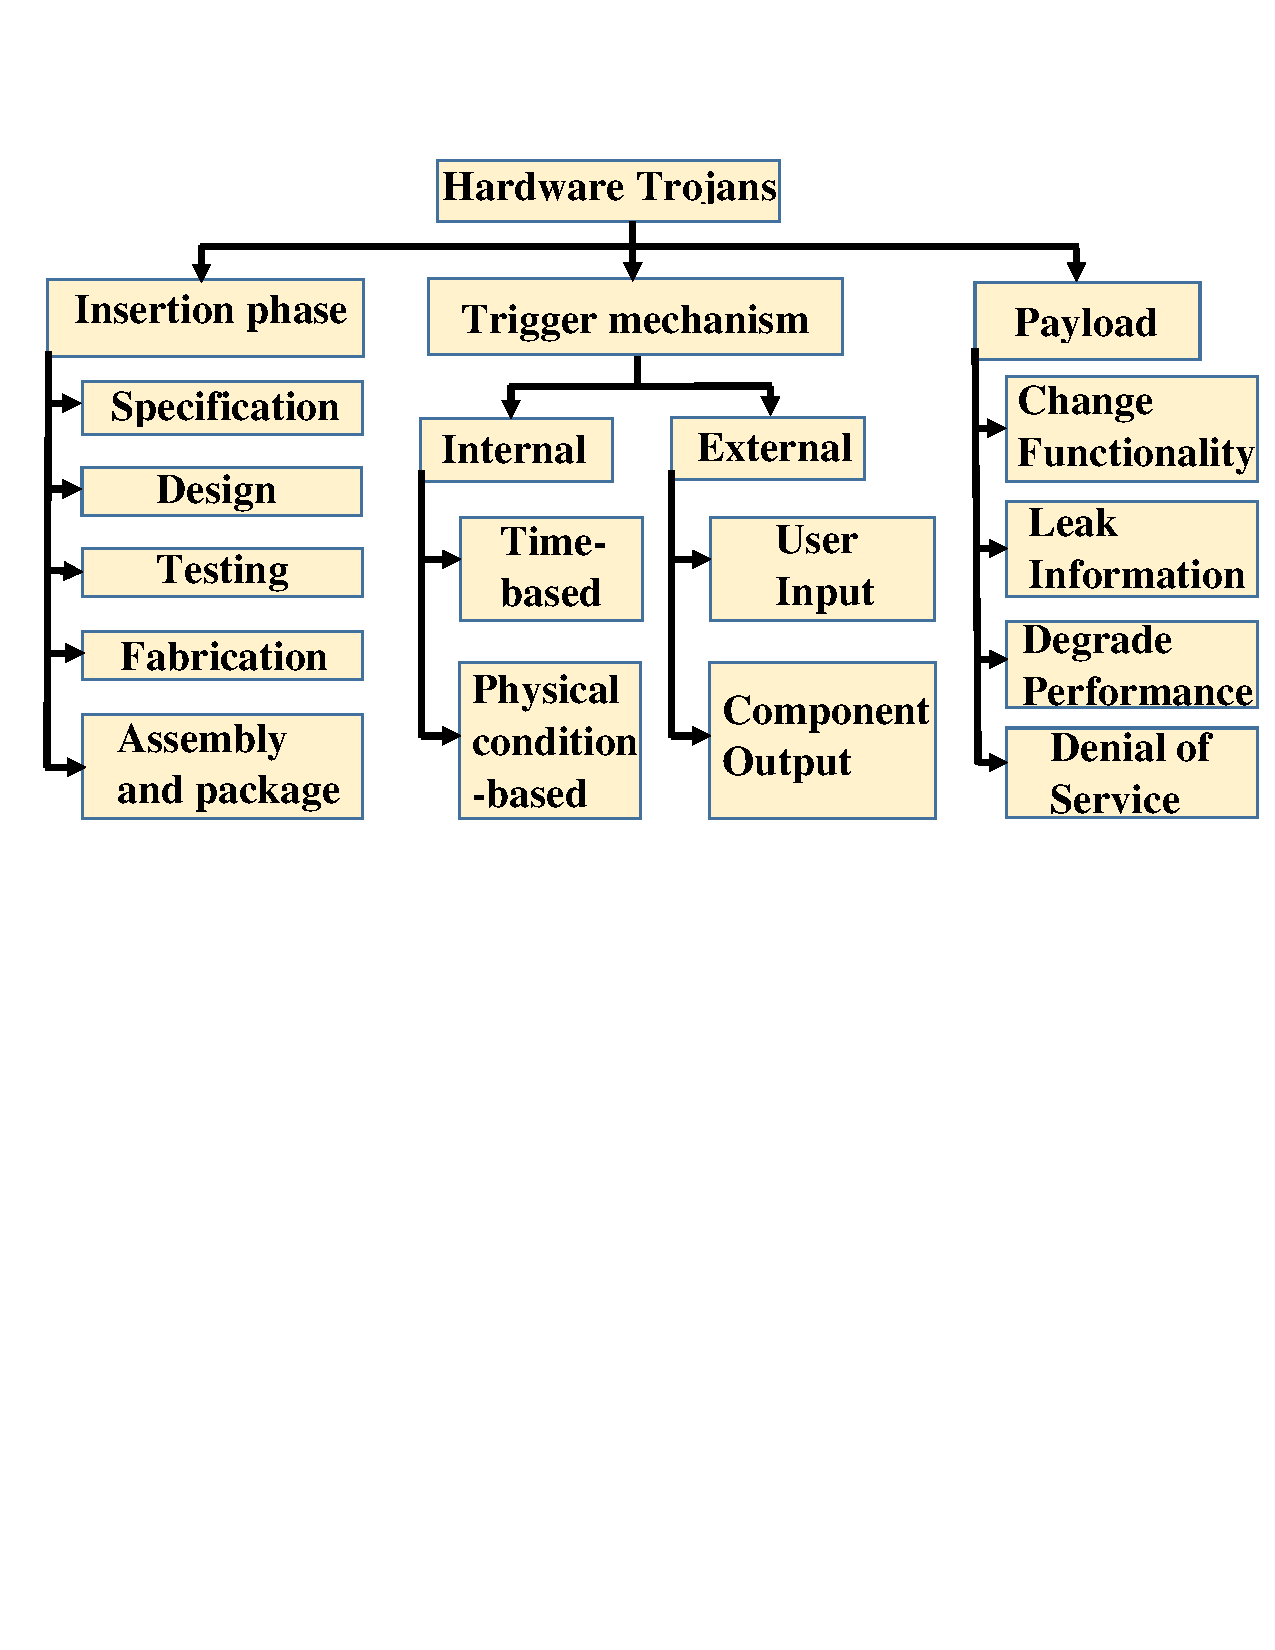
\includegraphics[viewport=0.1in 5.5in 21.3in 10in, clip,height=2.2in,width=9in,scale=1]{fig/HT_taxonomy.pdf}
	\caption{Hardware Trojans Taxonomy.}
	\label{fig:taxonomy}	
\end{figure}

\subsection{Backscattering Side-channel}
Backscattering side-channel is an impedance-based side-channel which is newly introduced in \cite{8701559}. Unlike other analog side-channels such as electromagnetic emanation (EM) and power which are the consequence of current flow change inside the chip, backscattering side-channel is an impedance-based side channel that is the consequence of impedance switching activities inside the chip. Backscattering side-channel can be created by propagating a continuous-signal toward the chip. The transistor switching activities cause the chip's impedance changes, which modify the radar cross-section (RCS) of the circuit. This RCS change modulates the signal that is backscattered from the chip, which creates an impedance-based backscattering side-channel. If hardware Trojan is added to a circuit, it changes the impedance of the circuit even if the Trojan is not activated. The changes will be reflected in the backscattered signal, which is beneficial to detection of hardware Trojan. That is why the backscattering side-channel is very effective and outperforms other side-channels for HT detection \cite{8701559}.

\section{Problem statement and attack models} \label{problem}

\section{A Novel Clustering Algorithm Using Backscattering Side-Channel} \label{agorithm}
\label{sec:identify}
\subsection{The affect of HTs on backscattering side-channel signal}
Most of digital circuits are synchronous, thus the overall switching pattern follows the clock cycle. The clock cycle usually accommodates switching delays along entire paths of logic gates, which means that the impedance changes of individual gates occur abruptly at some point in the clock cycle, i.e., they have a square-wave-like waveform. 
Therefore, the change caused by HTs will be reflected in backscattered signals at the circuit's clock harmonics: $f_{carrier} \pm f_c$, $f_{carrier} \pm 2*f_c$, etc. The first clock harmonics at $f_{carrier} \pm f_c$ will follow the overall RCS change during a cycle, while the remaining
harmonics will be affected by the rapidity (rise/fall times)
and timing of the impedance changes within the clock cycle.

As a result, backscattering approach relies on measuring the amplitude of the
back-scattered signal at the side-bands for the first $m$ harmonics of the clock frequency. Note that each clock harmonic produces two side-band
components that have the same amplitude, in this paper we
measure points to the right of the carrier, i.e. $f_{carrier} + f_c$,
$f_{carrier} + 2*f_c$, etc. These $m$ amplitudes measured for a given circuit form a
trace, and each trace characterizes the amount, duration, and timing of the circuit's impedance-change activity during a
clock cycle. Intuitively, by collecting
training traces using one or more genuine ICs, we can detect HTs on other ICs by collecting their traces and comparing them with the training traces.

However, the amplitude of a received signal declines rapidly
with distance. Fortunately, the distance affects all of the points in a trace
similarly, i.e., distance attenuates all amplitudes in the trace
by the same multiplicative factor. Therefore, rather than using
amplitudes for trace comparisons, we use amplitude ratios,
i.e., amplitude of a harmonic divided by the amplitude of the previous harmonic. This cancels out the trace's distance dependent
attenuation factor. The resulting $m - 1$ amplitude
ratios are then used for comparing traces.
\subsection{Clustering Algorithm For Backscattering Side-channel Using Graph Model}
This section provides the proposed methodology to identify the existence of Trojan injection. In that respect, let assume 
$$ {\bf y}_i = \left[  y_{i1} ~  y_{i2} ~ \cdots ~  y_{in} \right]$$
are the ratios of harmonics for the $i^{th}$ measurement, where $ y_{ij}$ is the ratio of $j^{th}$ and $(j + 1)^{th}$ harmonics of the $i^{th}$ board in dB. Moreover, let ${\bf Y}$ correspond the data matrix which can be written as
\begin{eqnarray}
{\bf Y} =  \left[\begin{array}{ccc}
\horzbar & {\bf y}_1 & \horzbar \\
\horzbar & {\bf y}_2 & \horzbar \\
&\vdots& \\
\horzbar & {\bf y}_m & \horzbar \\
\end{array}\right]
\end{eqnarray}
where $m$ is the number of measurements. The problem here  is that the size of the data can be large so that some of the crucial information can be hidden to identify Trojan injection. Therefore,
diminishing the size of the problem can eliminate the redundant information regarding the data. So, we first find the left singular vector of ${\bf Y} $, and project the data onto the space which is generated by some of the left singular vectors. These vectors correspond to singular values which contain  much of the energy of ${\bf Y}$. Assuming the singular value decomposition of  ${\bf Y}$ is ${\bf Y} = {\boldsymbol \Lambda \boldsymbol\Sigma  \boldsymbol V}^T$, we can write 
$${\bf A} = {\bf Y}^T{\bf Y} = \boldsymbol V \boldsymbol\Sigma^2 \boldsymbol V^T $$
where  ${\bf A} $ is the correlation matrix, and $\boldsymbol\Sigma^2$ corresponds to $\boldsymbol\Sigma^T\boldsymbol\Sigma$, which is also a diagonal matrix and contains the square of the singular values of ${\bf Y}$. 

Let assume the first $m$ singular values are the largest singular values  of the matrix ${\bf V}$,  and ${\bf V}_m$ be a sub-matrix with $m$ columns where columns correspond to these $m$ eigenvalues. 
%Let also $\boldsymbol\Sigma_m \in \Re e^{m\times m}$ be a diagonal matrix where the diagonal entries are these $m$ largest singular values. 
Therefore, to diminish the size of the data, we project ${\bf Y}$ into the column space of ${\bf V}_m$ as
\begin{equation}
{\bf Y}_P = {\bf Y} {\bf V}_m.
\end{equation} 
%where  $\boldsymbol \Sigma_m^{-1}$ is the inverse of $\boldsymbol \Sigma_m$. 
After discarding the redundant information, the next step is to find the clusters in the data. The expectation is that each cluster corresponds to differences between the boards due to production, or Trojan injection.  To find the clusters and corresponding centroid points, we use K-means algorithm. The number of clusters is chosen so that it is at least the number of different boards under inspection. However, having more than two clusters does not give enough information about the Trojan injection. To  detect existence of Trojan, the number of clusters must be at most two, which indicates one of the clusters belongs to the group with Trojan. 
%

To decrease the number of clusters, we propose to use graph method and shortest path algorithm. In that respect, we create a graph where each arc represents that two groups at the edges of the arc belong to same type. Here, our claim is that the type, which indicates the board is injected or not,  of two closest clusters are same if the distance of these clusters are below some threshold.  In other words, the constraint on arcs is that an arc is valid only if the distance between the clusters' centroids at the edges is small than a given threshold. The process for choosing the threshold is as follows: Let say after sorting the minimum distances, we obtain the vector ${\bf d}_v$, and the increase in the $i^{th}$ entry of the vector is more than 20\% comparing the $(i -1)^{st}$ entry. Then, we first set the threshold value as ${\bf d}_v[i-1]* 1.2$, and check whether the number of clusters is less than three.  If it is not, check the next entry, and follow the same procedure until having less than three groups. After, generating the graph and announcing the valid arcs, the last step is to exploit shortest path algorithm to check whether a node, i.e., a cluster, is reachable from another node. If there exists a path between these two nodes, we label these as the same type, otherwise, we claim there exists a group with Trojan. An example of the procedure is given in Section \ref{sec:experiment}. The method illustrates that the ratios of the harmonics help to identify the boards when a board is injected  with a Trojan.
\section{Evaluation} \label{evaluation}
\subsection{Experiment Setup}
The setup for experiments to evaluate the performance of the proposed algorithm is shown in Fig.~\ref{fig:meassetup}. The setup includes a transmitter Aaronia E1 electric-field near-field probe connected to an Agilent MXG N5183A Signal signal generator, and a receiver Aaronia H2 magnetic field near-field probe connected to an Agilent MXA N9020A spectrum analyzer. The devices-under-test (DuT) are Altera DE0 Cyclone V FPGA boards. An angle ruler is used as a positioner so that different DE0-CV boards can be tested using approximately the same position of probes. A laptop is used to control the devices and automate the measurements. A 3 GHz continuous sinusoid signal is generated by the signal generator and transmitted toward the FPGA chip using the transmitter probe. The backscattered signal is received by the receiver probe, and this signal are recorded by the spectrum analyzer.
\begin{figure}[htb]	
	\centering
	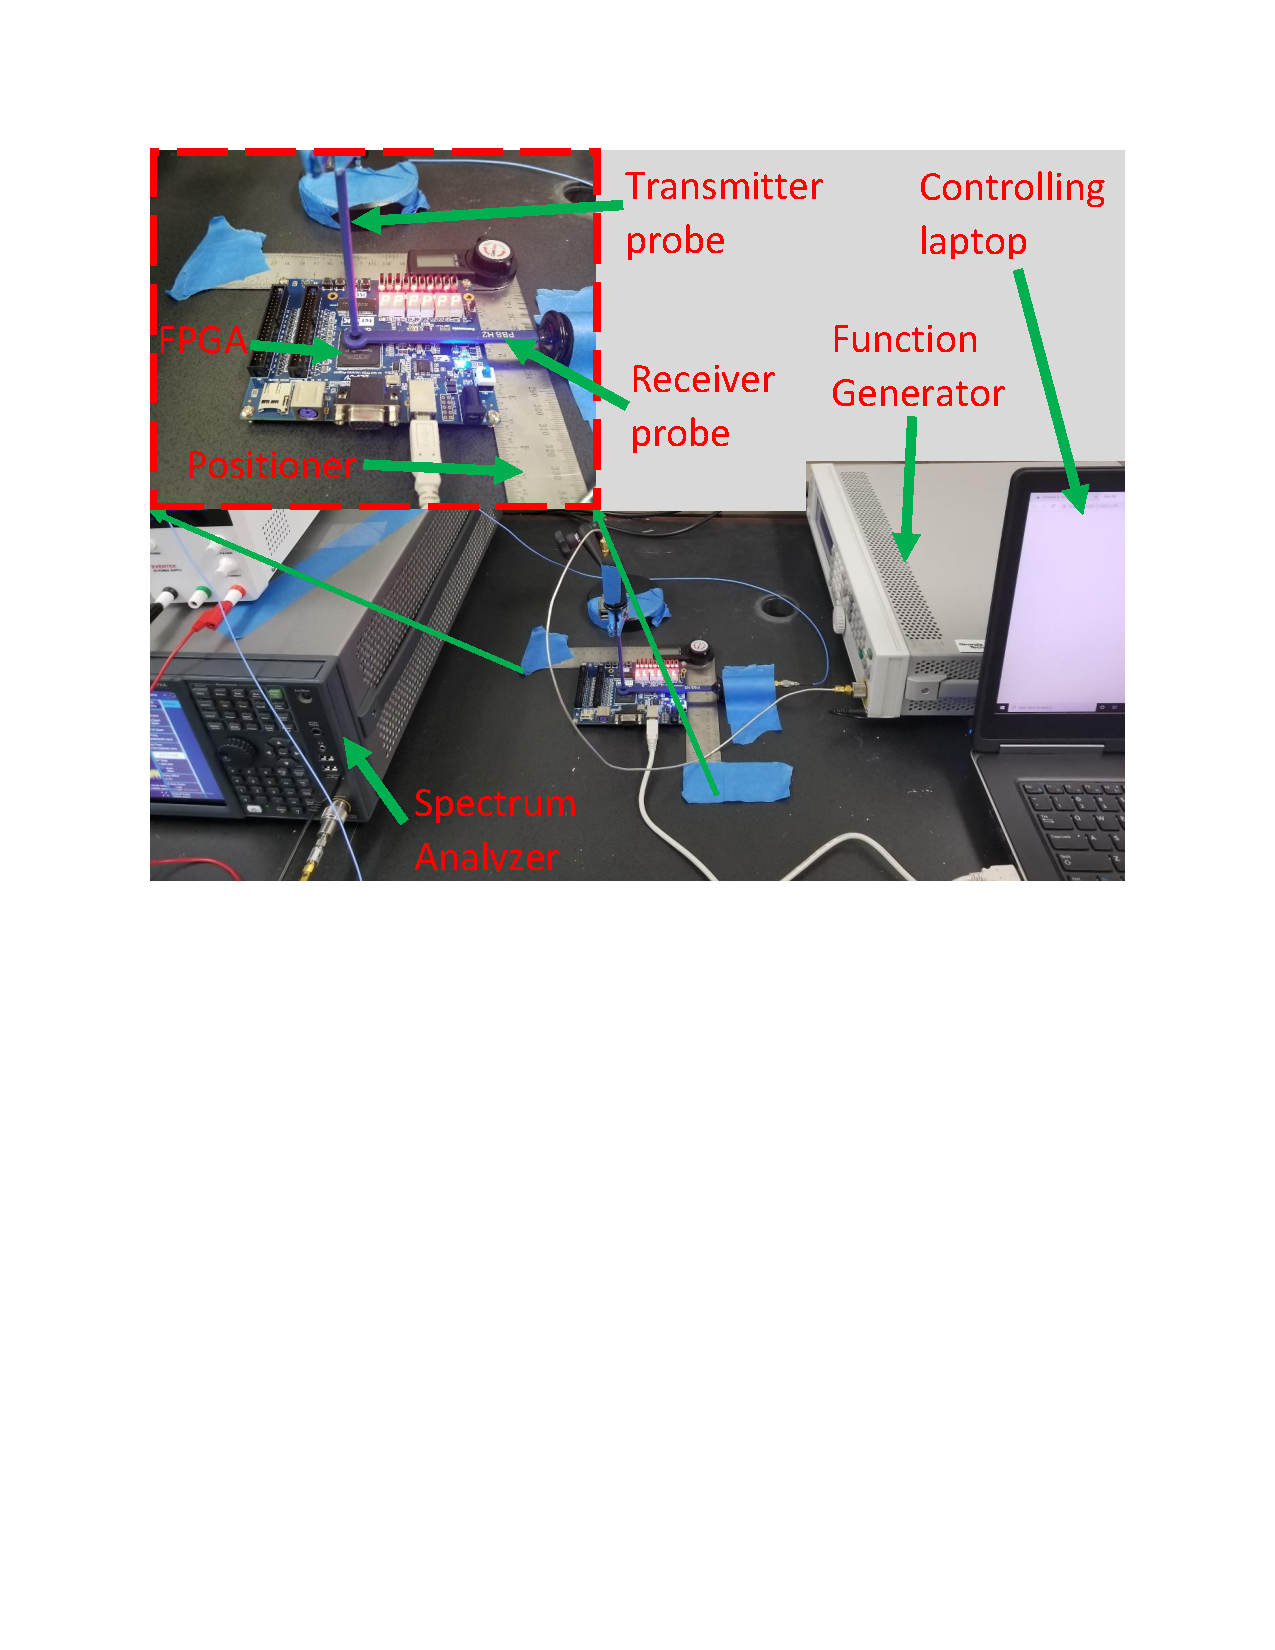
\includegraphics[viewport=1in 5in 16in 10in, clip,height=2.5in,width=8.1in,scale=1]{fig/measurement_setup_2.pdf}
	\caption{Measurement setup for hardware Trojan detection using IP side channel.}
	\label{fig:meassetup}	
\end{figure}
\subsection{Hardware Trojan Benchmark Implementation}
To evaluate our technique, we implement three
different benchmark circuits AES, RS232, and PIC16F84 the TrustHUB
Trojan repository \cite{Trusthub}. There are total 21 Trojan designs for AES circuit, 4 Trojan designs for PIC16F84 circuit, and 21 Trojan designs for RS232 circuit. Because numerous HTs in the TrustHub repository are similar to each other, we select ones that exhibit different approaches for their triggers and payloads as shown in Table \ref{table:benchmark}.

\bgroup
\def\arraystretch{1.5}%  1 is the default, change whatever you need
\begin{table}
	\centering
	\caption{Hardware Trojan Benchmarks and Detection Results}
	\begin{tabular}{|c|c|} 
		\hline
		\textbf{Benchmark} & \textbf{Size of Trojan} \\ 
		& \textbf{(Percentage of HT-free circuit)}  \\
			
		\hline
		AES-T500 & 1.79\% \\
		\hline
		AES-T400 & 2.03\% \\
		\hline
		AES-T700 & 1.88\% \\
		\hline
		PIC16F84-T100 & 3.15\% \\
		\hline
		PIC16F84-T200 & 3.28\% \\
		\hline
		PIC16F84-T400 & 3.10\% \\
		\hline
		RS232-T500 & 3.15\%  \\
		\hline
		RS232-T600 & 3.06\% \\
		\hline
		RS232-T700 & 3.02\% \\
		
		\hline
	\end{tabular}
	\label{table:benchmark}
\end{table}
\egroup

The Trojan-affected and Trojan-free designs are carefully mapped to the FPGA by using ECO ( Engineering Change Order) tools so that they have the same layout except for the Trojan part, thus making for a fair comparison. As mentioned in Section \ref{background}, it is extremely hard to activate a HT without priori knowledge of its triggering circuit, it is highly desirable for a HT detection technique to be able to detect HT when it is dormant. As a result, our evaluation will focus on evaluating our algorithm for dormant HTs. In other words, all Trojans stay inactive in all our experiments.

\subsection{Experimental Results}
\label{sec:experiment}
\subsubsection{Evaluation of Existing HT Benchmarks}
In this section, we provide the experimental results for Trojan detection. We first collect data from the boards with Trojan, and then without Trojan. We gather all the data in  ${\bf Y}$. Here, we need to note that although we know the labels for each experiment, for the analysis purposes we assume we do not know the types of each board. 

The first step is to find the left singular value of the measurement matrix ${\bf Y}$. For that, we calculate the eigenvalues of ${\bf A}$, and then corresponding ${\bf V}_m$.  To visually see the data, we choose $m=3$.  Fig. \ref{fig:groundTruth} provides the data after projection to the space defined by  ${\bf V}_3$. 

\begin{figure}[ht]
	\centering
	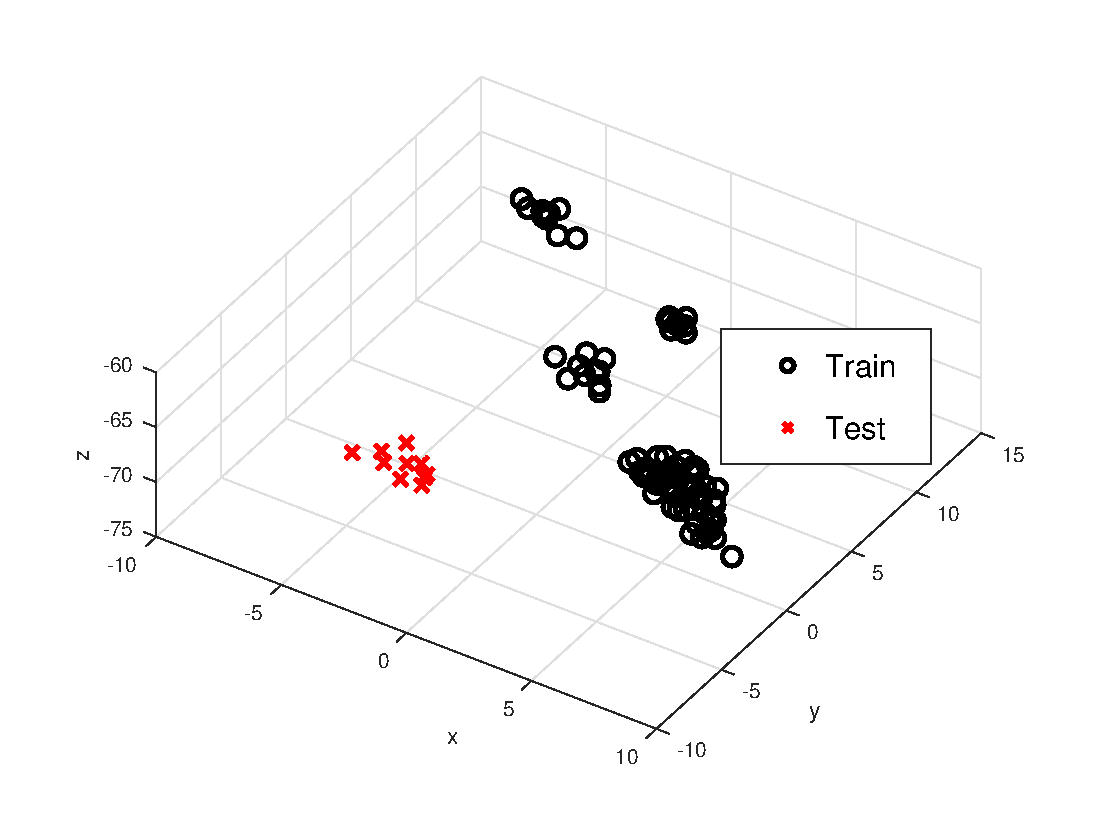
\includegraphics[trim=0.0in 0.0in 0.0in 0.0in,clip=true,width=\linewidth]{figure/originalGraph.eps}
	\caption{Ground truth information for the  boards.}
	\label{fig:groundTruth}
\end{figure}

The number of measurements for the boards with Trojan is  70, and for the boards without Trojan is 90. We observe that although we only have one cluster for the data with Trojan, we have multi-clusters for the data without Trojan. Actually, this could give the intuition that  the effect of the Trojan on the magnitudes of the harmonics of the clock cycles dominates the differences caused by                           the production. ({\bf To be able to claim that, we need more measurement actually.})



\begin{figure}[ht]
	\centering
	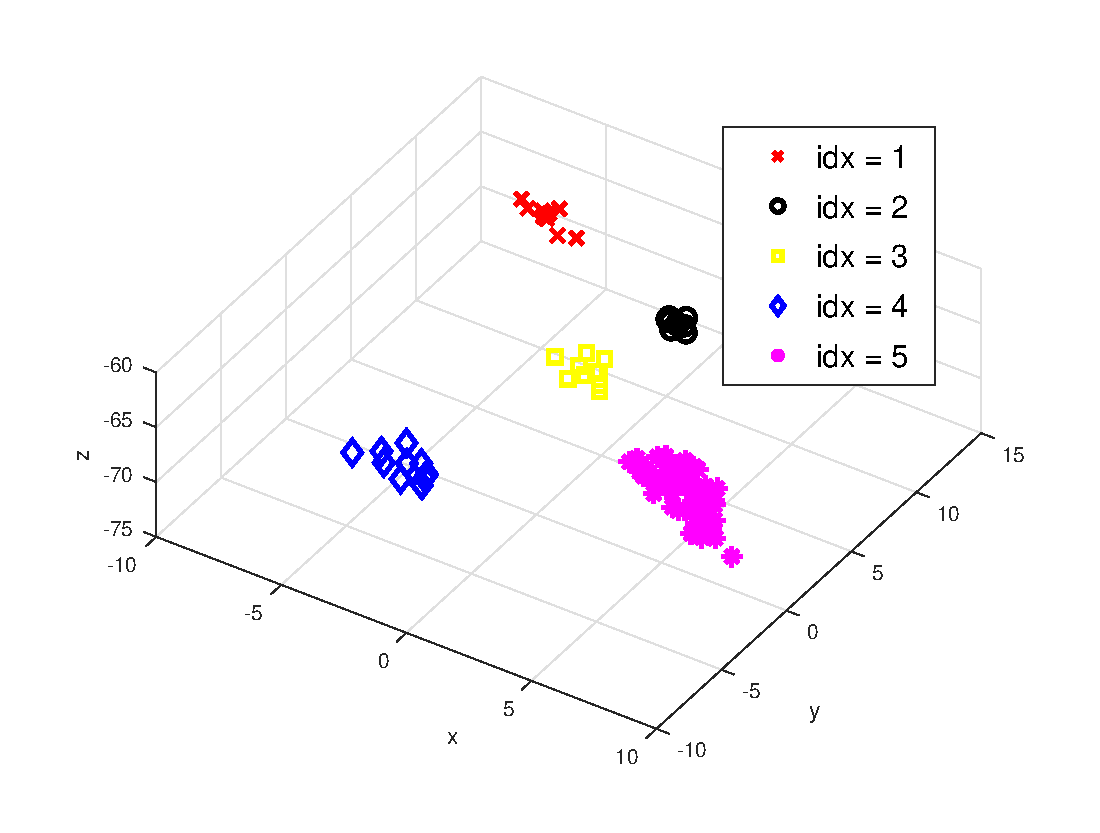
\includegraphics[trim=0.0in 0.0in 0.0in 0.0in,clip=true,width=\linewidth]{figure/kmeansResult.eps}
	\caption{K-means clustering of the boards when the number of center points is chosen as five.}
	\label{fig:kmeans}
\end{figure}

However, since our assumption is that we do not have the labels for the measurements, we first apply K-means algorithm with 5 clusters. The result of the algorithm is given in Fig. \ref{fig:kmeans}. We observe that there exist five distinct groups. The problem here is that these clusters are results of differences in production or injection of a Trojan, but we need more information for the cause of these distinct clusters. Therefore, the next step is to apply the graph method. In that respect, we first calculate the distances among all centroids. We choose threshold by considering the minimum distance from each node to  others, and that the number of clusters is not more than two.  In that respect, we first sort the distance, and then seek for a gap among sorted values as explained in Section \ref{sec:identify} to set the threshold value.

\begin{figure}[ht]
	\centering
	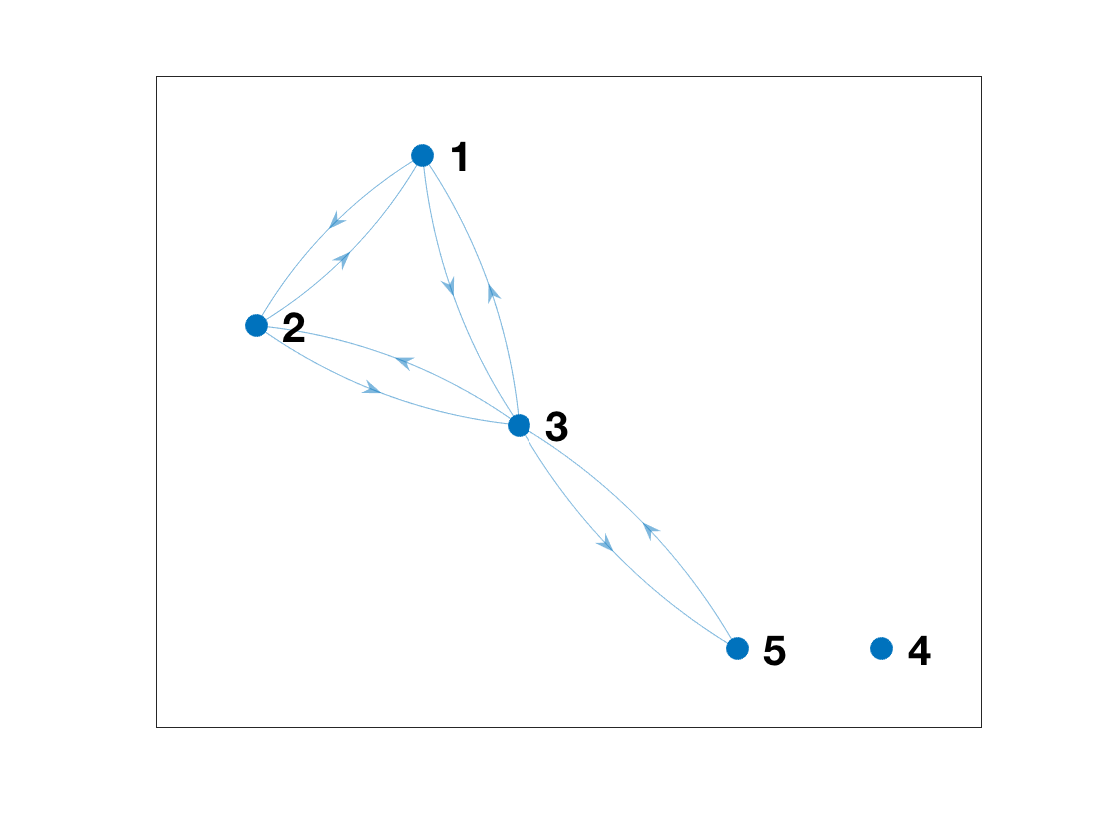
\includegraphics[trim=0.0in 0.0in 0.0in 0.0in,clip=true,width=\linewidth]{figure/graphPlot.eps}
	\caption{Generation of the graph based on the distances between the centroids of the clusters.}
	\label{fig:graph}
\end{figure}

After setting the threshold, we obtain the graph given in Fig. \ref{fig:graph}. In the figure, nodes correspond to groups and arcs represent the paths where the distances between nodes are below the threshold value. We observe that there exist two different groups since the group with label 4 is not reachable from any other nodes. As the final step, to divide all clusters into two groups, we apply shortest path algorithm to find which nodes are connected. The results are given in Fig. \ref{fig:clusters}. The observation is that there exist  two different groups which indicates the possible Trojan injection into some of the boards. 

\begin{figure}[ht]
	\centering
	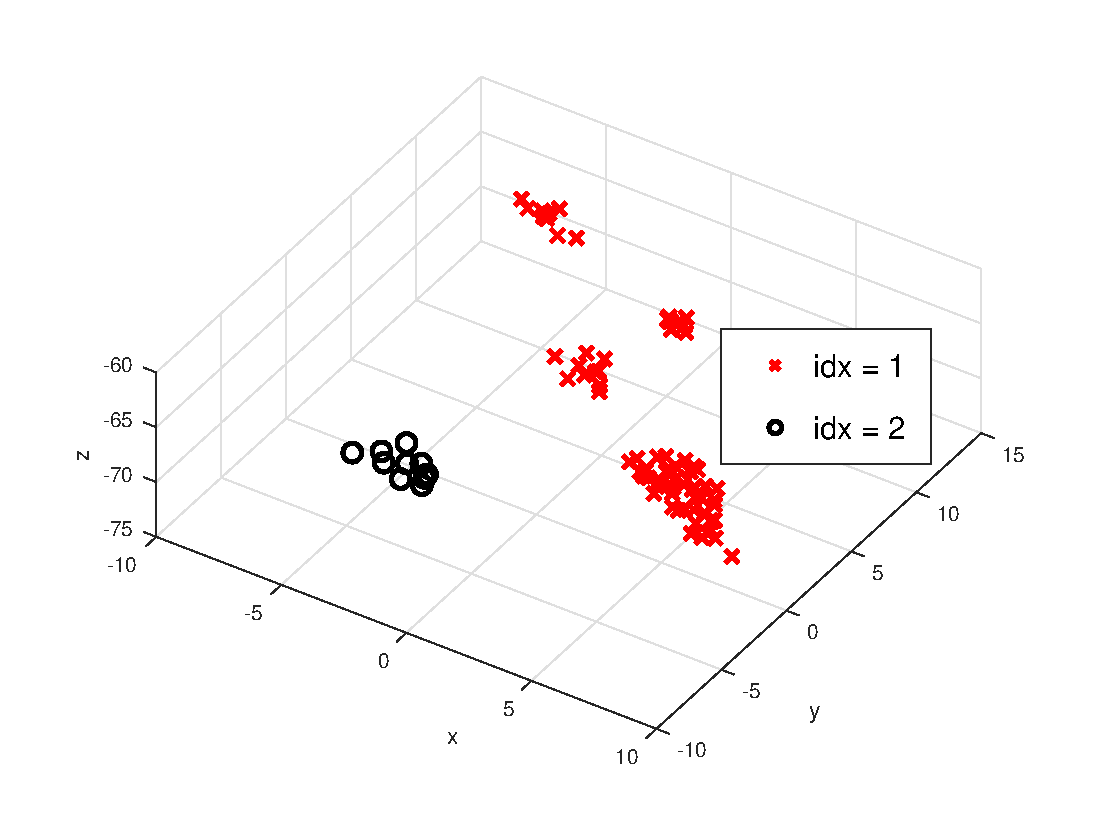
\includegraphics[trim=0.0in 0.0in 0.0in 0.0in,clip=true,width=\linewidth]{figure/clusteringResult.eps}
	\caption{Clustering the data into two groups as Trojan injected vs. no-Trojan.}
	\label{fig:clusters}
\end{figure}
\subsubsection{Evaluation of Changing Size of Hardware Trojans}
Because the algorithm performs so well on the existing HT designs in Table \ref{table:benchmark}, this Section focuses on testing the limit of our algorithm by reducing the size of HTs. The RS232-T500 is chosen for this experiment because both its payload and its trigger can be meaningfully resized. As a result, we have HT benchmarks as summarized in Table \ref{table:size}.

\bgroup
\def\arraystretch{1.5}%  1 is the default, change whatever you need
\begin{table}
	\centering
	\caption{Hardware Trojan Benchmarks and Detection Results}
	\begin{tabular}{|c|c|} 
		\hline
		\textbf{Benchmark} & \textbf{Size of Trojan} \\ 
		& \textbf{(Percentage of HT-free circuit)}  \\
		
		\hline
		RS232-T500 w/ 1/2 size  & 1.74\%  \\
		\hline
		RS232-T500 w/ 1/4 size & 0.97 \% \\
		\hline
		RS232-T500 w/ 1/8 size & 0.51\% \\
		
		\hline
	\end{tabular}
	\label{table:size}
\end{table}
\egroup


\bibliographystyle{IEEEtran}
\bibliography{bare_jrnl}


% if have a single appendix:
%\appendix[Proof of the Zonklar Equations]
% or
%\appendix  % for no appendix heading
% do not use \section anymore after \appendix, only \section*
% is possibly needed

% use appendices with more than one appendix
% then use \section to start each appendix
% you must declare a \section before using any
% \subsection or using \label (\appendices by itself
% starts a section numbered zero.)
%

% Can use something like this to put references on a page
% by themselves when using endfloat and the captionsoff option.
\ifCLASSOPTIONcaptionsoff
  \newpage
\fi



% trigger a \newpage just before the given reference
% number - used to balance the columns on the last page
% adjust value as needed - may need to be readjusted if
% the document is modified later
%\IEEEtriggeratref{8}
% The "triggered" command can be changed if desired:
%\IEEEtriggercmd{\enlargethispage{-5in}}

% references section

% can use a bibliography generated by BibTeX as a .bbl file
% BibTeX documentation can be easily obtained at:
% http://mirror.ctan.org/biblio/bibtex/contrib/doc/
% The IEEEtran BibTeX style support page is at:
% http://www.michaelshell.org/tex/ieeetran/bibtex/
%\bibliographystyle{IEEEtran}
% argument is your BibTeX string definitions and bibliography database(s)
%\bibliography{IEEEabrv,../bib/paper}
%
% <OR> manually copy in the resultant .bbl file
% set second argument of \begin to the number of references
% (used to reserve space for the reference number labels box)
%%\begin{thebibliography}{1}

%\bibitem{IEEEhowto:kopka}
%H.~Kopka and P.~W. Daly, \emph{A Guide to \LaTeX}, 3rd~ed.\hskip 1em plus
 % 0.5em minus 0.4em\relax Harlow, England: Addison-Wesley, 1999.

%\end{thebibliography}

% biography section
%
% If you have an EPS/PDF photo (graphicx package needed) extra braces are
% needed around the contents of the optional argument to biography to prevent
% the LaTeX parser from getting confused when it sees the complicated
% \includegraphics command within an optional argument. (You could create
% your own custom macro containing the \includegraphics command to make things
% simpler here.)
%\begin{IEEEbiography}[{\includegraphics[width=1in,height=1.25in,clip,keepaspectratio]{mshell}}]{Michael Shell}
% or if you just want to reserve a space for a photo:

\begin{IEEEbiography}[{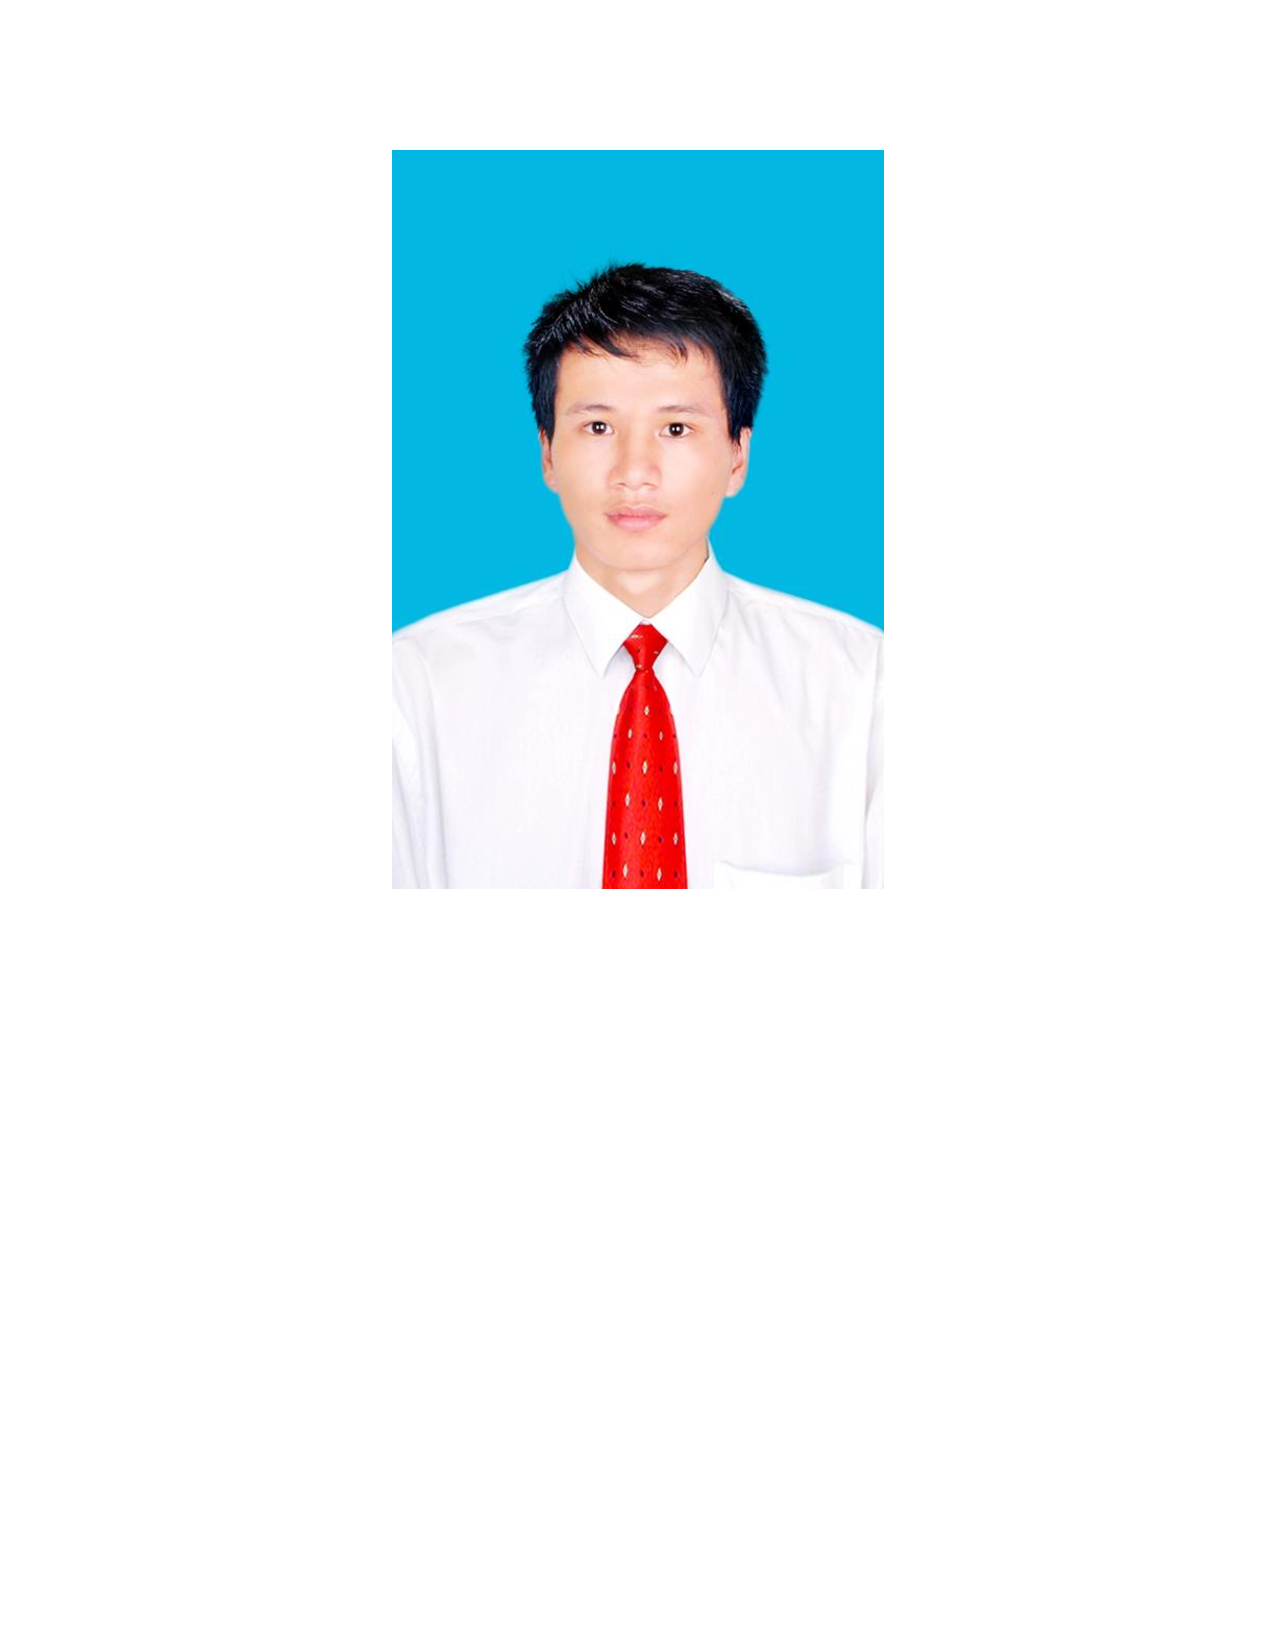
\includegraphics[viewport=2.52in 5.22in 8.47in 9.2in,width=1.85 in,height=1.25 in,clip]{fig/photo_pavel.pdf}}]
	{Luong N. Nguyen} (S'18) received
	the B.Sc. degree in Electrical and Computer Engineering from the Hanoi University of Science and Technology in 2013 and
	the M.Sc. degree in Electrical and Computer Engineering from the Seoul National University in 2016.
	Since 2016, he has been a Graduate Research Assistant, pursuing the Ph.D. degree in the School of Electrical and Computer Engineering,
	Georgia Institute of Technology focusing on digital circuit design, software and hardware security, and embedded system.
	His current research interests span areas of ASIC design, computer architecture, and electrical engineering.
	He is a past recipient of the Korean Government Scholarship Program, and the best paper award from the 2014 Korean SoC conference.
\end{IEEEbiography}

\begin{IEEEbiography}[]
	{Baki Berkay Yilmaz} (S’16) received the B.Sc. and 	M.Sc. degrees in Electrical and Electronics Engineering from Koc University, Turkey in 2013 and 2015 respectively. He joined Georgia Institute of Technology in Fall 2016 and he is currently pursuing his PhD in School of Electrical and Computer Engineering, focusing on quantifying covert/side-channel information leakage and capacity. Previously, he worked on channel equalization and sparse reconstruction. His research interests span areas of electromagnetic, signal processing and information
	theory.
\end{IEEEbiography}

\begin{IEEEbiography}[{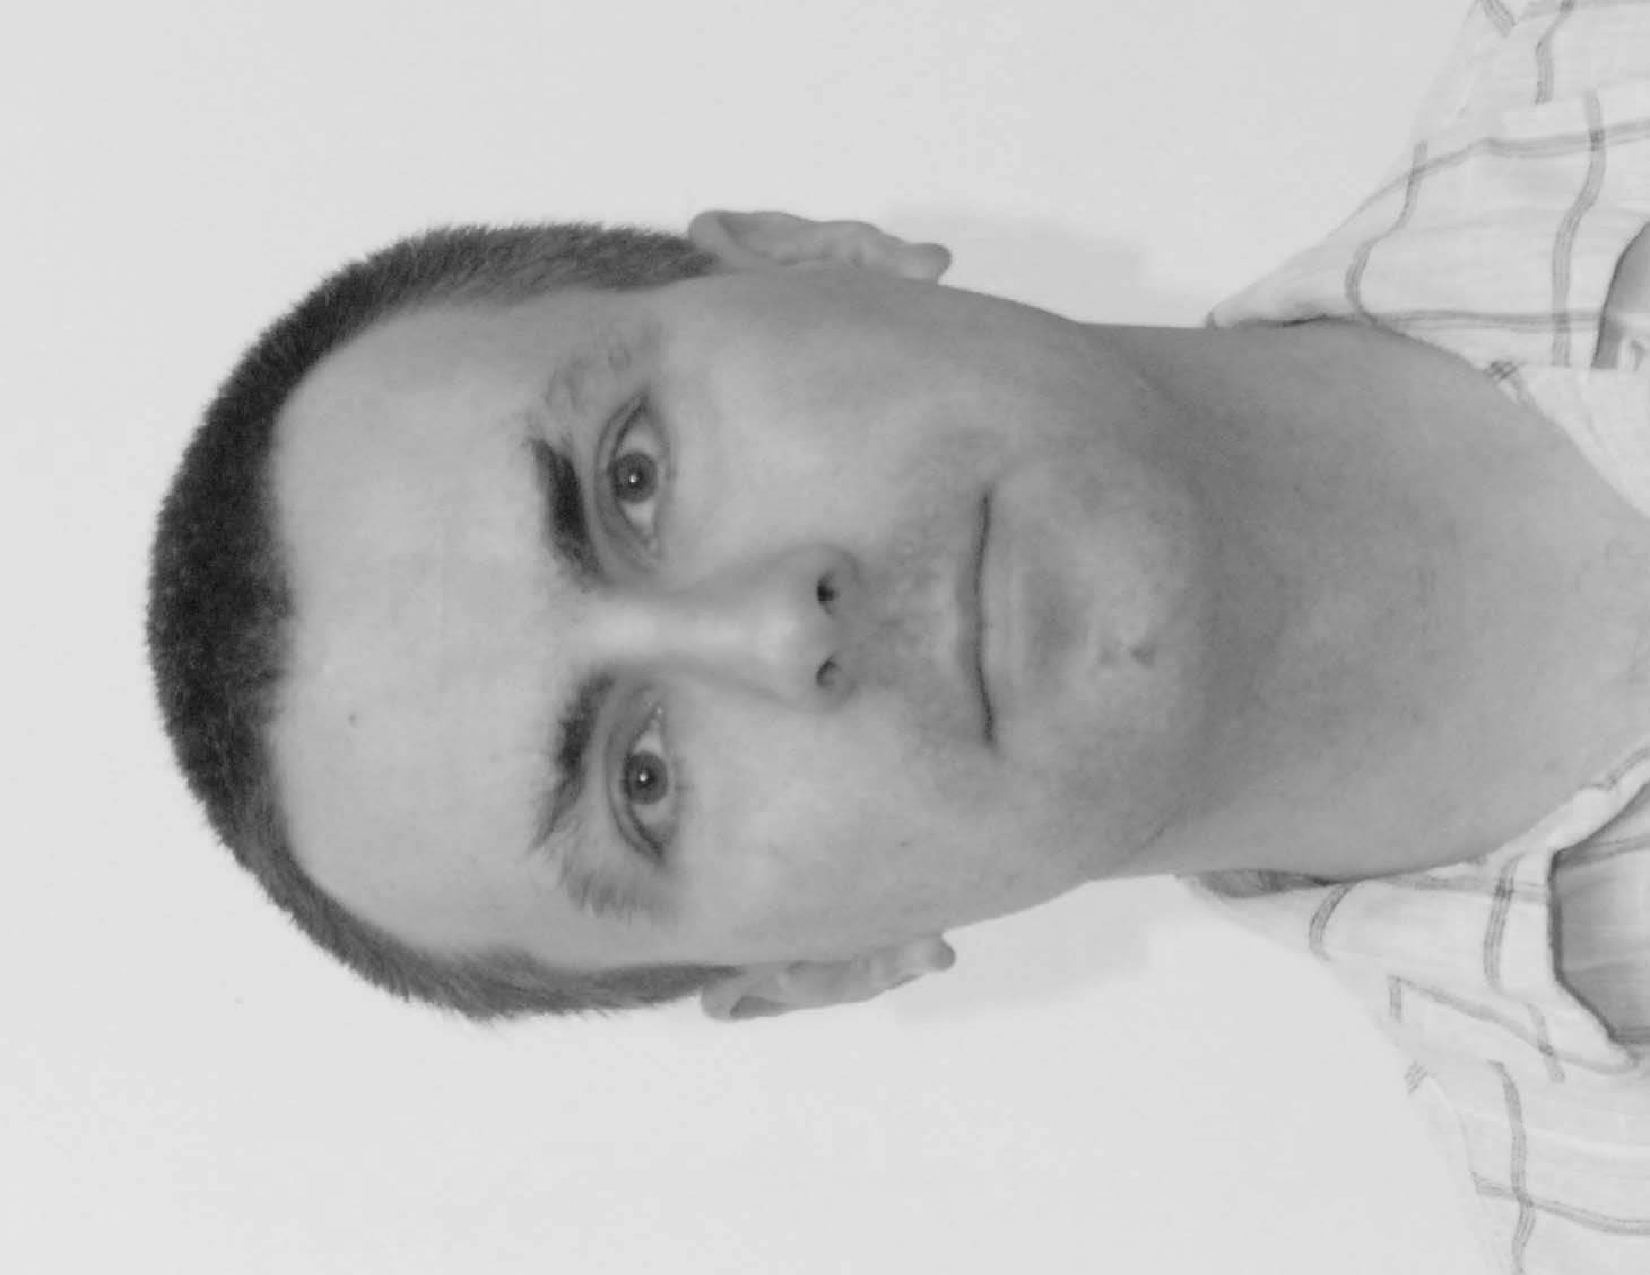
\includegraphics[width=1.25 in,height=1 in,clip,angle=270]{fig/photo_milos.pdf}}]{Milos Prvulovic} (S'97-M'03-SM'09) received the B.Sc. degree in electrical engineering from the University of Belgrade in 1998, and the M.Sc. and Ph.D. degrees in computer science from the University of Illinois at Urbana-Champaign in 2001 and 2003, respectively. He is a Professor in the School of Computer Science at the Georgia Institute of Technology, where he joined in 2003. His research interests mainly focus on the interaction between computer architecture, computer system security, and software engineering.
	
Dr. Prvulovic is recipient of the following awards/honors: NSF CAREER Award (2005), Best Paper Award at the 49th Annual IEEE/ACM International Symposium on Microarchitecture, 2016, and Distinguished Alumni Educator Award, 2012, from the Department of Computer Science at the University of Illinois at Urbana-Champaign.
\end{IEEEbiography}
\vspace{-0.2in}
\begin{IEEEbiography}[{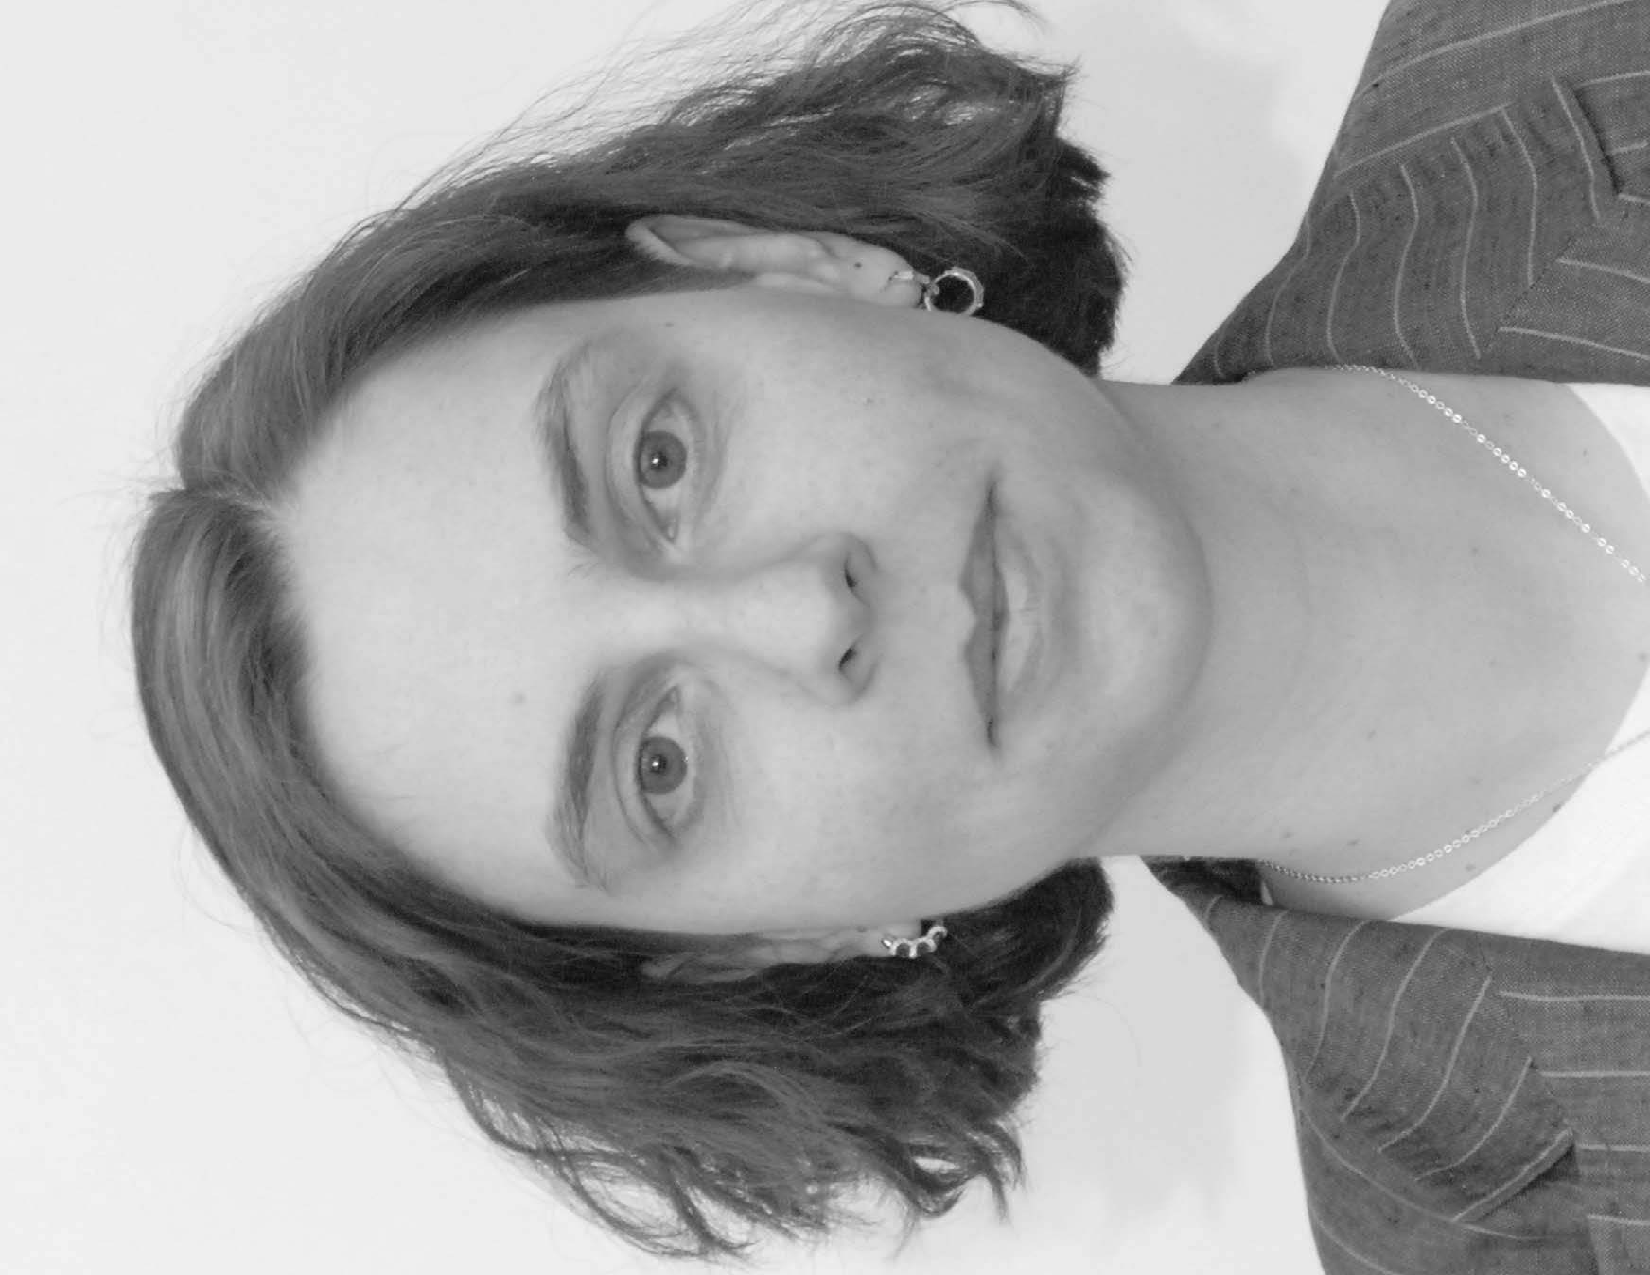
\includegraphics[width=1.25 in,height=1 in,clip,angle=270]{fig/photo_alenka.pdf}}]{Alenka~Zaji\'{c}} (S'99-M'09-SM'13)
	received the B.Sc. and M.Sc. degrees form the School of Electrical Engineering, University of Belgrade, in 2001 and 2003, respectively. She received her Ph.D. degree in Electrical and Computer Engineering from the Georgia Institute of Technology in 2008. Currently, she is an Associate Professor in the School of Electrical and Computer Engineering at Georgia Institute of Technology. Her research interests span areas of electromagnetics, wireless communications, signal processing, and computer engineering.
	
	Dr. Zaji\'{c} is the recipient of the following awards: NSF CAREER Award (2017), Best Paper Award at the 49th Annual IEEE/ACM International Symposium on Microarchitecture, 2016, 2012 Neal Shepherd Memorial Best Propagation Paper Award, the Best Student Paper Award at the IEEE International Conference on Communications and Electronics 2014, the Best Paper Award at the International Conference on Telecommunications 2008, the Best Student Paper Award at the 2007 Wireless Communications and Networking Conference, LexisNexis Dean's Excellence Award 2016, and Richard M. Bass/Eta Kappa Nu Outstanding Teacher Award 2016. She has been an editor for IEEE Transactions on Wireless Communications 2012-2017.
	
\end{IEEEbiography}

% You can push biographies down or up by placing
% a \vfill before or after them. The appropriate
% use of \vfill depends on what kind of text is
% on the last page and whether or not the columns
% are being equalized.

%\vfill

% Can be used to pull up biographies so that the bottom of the last one
% is flush with the other column.
%\enlargethispage{-5in}


% that's all folks
\end{document}


